\chapter{Results and Discussions}\label{ch:results}
This chapter is organized as follows: Section \ref{sec:result_data} will discuss the main data used in this study, including an illustration of how to access it and the features it provides; Section \ref{sec:ch4_desc_stat} will discuss the results of the descriptive statistics; Section \ref{sec:ch4_morphological_analysis} will discuss the results on the morphological analyses; Section \ref{sec:ch4_structural_analysis} will discuss the results on the structural analyses; Section \ref{sec:ch4_topic_modeling_result} will discuss the results of the topic modeling; and Section \ref{sec:ch4_relating_islamic_texts} will discuss the results of relating the Qur'\=an to other Islamic texts and analyses. Finally, Section \ref{sec:ch4_limitations} will discuss the limitations of the models used in this study.
\section{Theoretical Results}
The different analyses provided in this chapter were based on theoretical results of this paper, all of which are original contribution and are provided in the appendices. It will be discussed separately in the appendices to avoid cluttering this chapter with heavy mathematics that many Islamic scholars may not be familiar with. These results are provided in the appendices for reviewers and readers to see the details of the math behind the analyses.
\section{Qur'\=an Data}\label{sec:result_data}
The main data used in this study is the digitized Qur'\=an data available through QuranTree.jl library by \citeA{asaad2021qurantree}. QuranTree.jl has both the Tanzil data\footnote{\url{https://tanzil.net/}} and the Qur'anic Arabic Corpus\footnote{\url{https://corpus.quran.com/}}, where the latter contains the morphological data of the Qur'\=an. These digital data will help in doing programmatic analyses of the Qur'\=an using Julia programming language. To see how to access this in QuranTree.jl in Julia, Figure \ref{fig:result_crps_tbl} shows the code for accessing the morphological data of the first \arb[trans]{'ayaT} \arb{'ayaT} of \arb[trans]{sUraTu 'l-fAti.haT} \arb{sUraTu 'l-fAti.haT}. Note that, the setup on how to install the said QuranTree.jl and other libraries and the Julia programming language is given in Appendix \ref{appendix:installation_libraries}.

Referring to Figure \ref{fig:result_crps_tbl}, the first line of the code, which has the code \texttt{using QuranTree}, loads the QuranTree library. The second line, which has the code \texttt{crps, tnzl = load(QuranData())}, loads both the morphological data and the Tanzil data of the Qur'\=an. The third line of the code converts these data into a tabular form. Finally, the fourth line of the code queries the first \arb[trans]{sUraT} \arb{sUraT} and the first \arb[trans]{'ayaT} \arb{'ayaT} of the morphological data of the Qur'\=an, the results of which are shown in succeeding lines with the heading indicating \texttt{Chapter 1} and \texttt{Verse 1}. Both the number 1 for Chapter 1 is indicated by \texttt{[1]} and \texttt{[1]}, respectively, in the code \verb|crps_tbl[1][1]| in Figure \ref{fig:result_crps_tbl}.

\begin{figure}[!t]
    \centering
    \includegraphics[width=\textwidth]{img/crps_tbl.png}
    \caption{\arb[trans]{sUraTu 'l-fAti.haT} \arb{sUraTu 'l-fAti.haT} morphological data}
    \label{fig:result_crps_tbl}
\end{figure}

The output of the code in Figure 1 as indicated by the lines starting with \texttt{\#} shows the morphological data of the \textit{basmallah} \arb[fullvoc]{bismi 'l-l_ahi 'l-ra.hm_ani 'l-ra.hImi}. In this data, there are five columns after the Row column. The \texttt{word} column indicates the word of the queried data, in this case the first \arb[trans]{'ayaT} \arb{'ayaT} of the first \arb[trans]{sUraT} \arb{sUraT}. According to this column, there are four words in the \textit{basmallah}. The second column, \texttt{part}, indicates the parts of the word. In this case, the first word, has two parts. These two parts is indicated by its \texttt{form} in the third column, which are \texttt{bi} a Roman encoding based on Buckwalter mapping which is decoded in Arabic as \arb{bi}, and the second part of the first word has the form in Roman encoding through Buckwalter as \texttt{somi} or decoded in Arabic as \arb[fullvoc]{smi}. The fourth column indicates the part-of-speech of the parts of the words. For the first word, \arb[fullvoc]{bismi}, its two parts are composed of Preposition \arb{bi} and a Noun \arb[fullvoc]{smi}, both of which are further described in the \texttt{features} column, which is the morphological features column. In this last column, it further tells the reader that the Preposition \arb{bi} is a prefix. In addition, the second part \arb[fullvoc]{smi} is the stem of the word \arb[fullvoc]{bismi}, with lemma indicated by \texttt{\{som} which is decoded as \arb{"ism}, and a root of \arb{smw}. There are still other features detailed in the morphological column for the second word \arb[fullvoc]{smi}, and this can be describe further using QuranTree.jl's \texttt{@desc} macro. The result of which is given in Figure \ref{fig:result_at_desc_basmallah}, which also show the other features such as the gender of the noun, in this case it is Masculine and is in Genitive case.

\begin{figure}[!t]
    \centering
    \includegraphics[width=\textwidth]{img/at_desc_basmallah.png}
    \caption{Morphological feature of the second part of the word \arb[fullvoc]{bismi}}
    \label{fig:result_at_desc_basmallah}
\end{figure}

The Quranic Arabic Corpus data which contain the morphological features discussed above, has the Qur'\=an texts represented as Buckwalter encoding, which is a character by character mapping of the Arabic orthographies of the Qur'\=an into a Roman letter. This encoding if decoded to Arabic matches exactly the Qur'\=an musaf. In fact, the Tanzil data which is also available in QuranTree.jl, exactly matches this data. The difference between the two is that the Tanzil data only contains the Arabic texts of the Qur'\=an broken down up until the \arb[trans]{'ayaT} \arb{'ayaT} only. Figure \ref{fig:result_tnzl_tbl} shows the Tanzil data queried through the QuranTree.jl for \arb[trans]{sUraTu 'l-fAti.haT} \arb{sUraTu 'l-fAti.haT}. The only difference between the two data in terms of presentation of the \arb[trans]{sUraT} \arb{sUraT} is that, the Quranic Arabic Corpus (in Figure \ref{fig:result_crps_tbl}) skips the \textit{basmallah} for all \arb[trans]{sUwar} \arb{sUwar} except for the first, \arb[trans]{sUraTu 'l-fAti.haT} \arb{sUraTu 'l-fAti.haT}, while the Tanzil data has it in every \arb[trans]{sUwar} \arb{sUwar}.

\begin{figure}[!t]
    \centering
    \includegraphics[width=\textwidth]{img/tnzl_tbl.png}
    \caption{\arb[trans]{sUraTu 'l-fAti.haT} \arb{sUraTu 'l-fAti.haT} Tanzil data}
    \label{fig:result_tnzl_tbl}
\end{figure}

The rich data available in QuranTree.jl opens up many possibilities for researchers to do programmatic analyses of the Qur'\=an. Especially on the use of Statistical modeling to understand its structure and patterns. This paper will demonstrate some of these possibilities. The data can be used to do morphological analyses, structural analyses, and even topic modeling. The data can also be used to do other analyses such as sentiment analysis, and other text analytics. 

\section{Descriptive Statistics}\label{sec:ch4_desc_stat}
The first statistical analysis is to describe the distribution of the data, through Descriptive Statistics. This statistical method is mainly used to summarize the data by looking at the central tendency, dispersion, and shape of the distribution of the data. The central tendency is a measure of the center of the data, which can be represented by the mean, median, and mode. The dispersion is a measure of how spread out the data is, which can be represented by the range, variance, and standard deviation.

The data in this case are the orthographies, parts of words, words, \arb[trans]{ayAt} \arb{ayAt}, and \textit{s\=urah} \arb{sUraT} of the Qur'\=an. The Qur'\=an is a collection of 114 \textit{s\=urah} \arb{sUraT} and 6,348 \arb[trans]{ayAt} \arb{ayAt}. Each \textit{s\=urah} \arb{sUraT} is made up of a number of \arb[trans]{ayAt} \arb{ayAt}, and each \arb[trans]{ayAt} \arb{ayAt} is made up of a number of words, which in turn is made of parts, and finally parts are made up of Arabic letters. These data as discussed in the previous section are available through the Quranic Arabic Corpus and the Tanzil data in the QuranTree.jl library.

As discussed in the Introduction of this thesis, the Qur'\=an has unique organizational structure unlike other scriptures. This has attracted both Muslims and non-Muslims to endeavor on understanding its structure. Most of the scholars have done this manually, going through each \arb[trans]{ayAt} \arb{ayAt} and \arb[trans]{sUraT} \arb{sUraT} of the Qur'\=an one at a time to find patterns that will at least convey why it is arranged as it is. However, this manual process is very tedious and time consuming, and hence other opportunities to understanding its structure has not yet been explored. Among those is undersanding the statistics of the counts of the words, \arb[trans]{AyAt} \arb{AyAt}, and \arb[trans]{suwar} \arb{suwar}. 

\begin{figure}[!t]
    \centering
    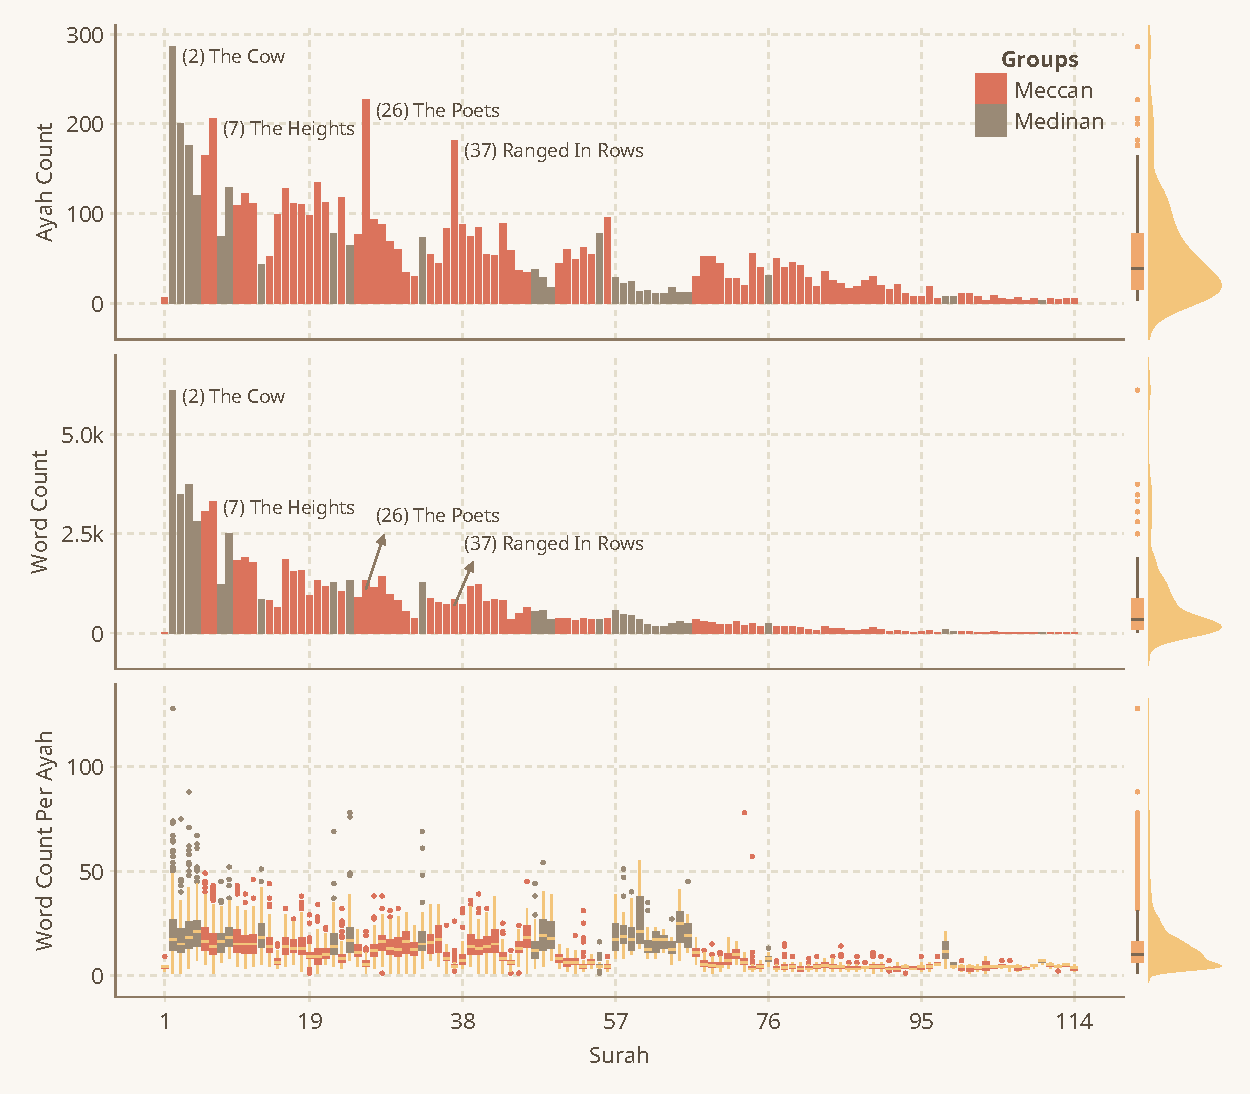
\includegraphics[width=\textwidth]{img/plot1.pdf}
    \caption{Distribution of Meccan and Medinan \arb[trans]{sUwar} \arb{sUwar}}
    \label{fig:result_ayah_word_count}
\end{figure}

Figure \ref{fig:result_ayah_word_count} shows the bar chart of the \arb[trans]{AyAt} \arb{AyAt} counts and word counts, and also the distribution of the word counts and character counts both per \arb[trans]{ayAt} \arb{ayAt}. In this figure, the geographical locations (Meccan or Medinan) of the \arb[trans]{sUraT} \arb{sUraT} based on the \arb[trans]{'asbAb 'alnuzUl} \arb{'asbAb 'alnuzUl} or the 'occasions/circumstances of revelation' are also indicated.

The first obvious pattern, which is known to Muslims, is the monotonically decreasing number of the \arb[trans]{ayAt} \arb{ayAt} after the first \arb[trans]{sUraT} \arb{sUraT}. This is true for both the bar charts of the \arb[trans]{ayAt} \arb{ayAt} count and the word count. An interesting pattern also is that, two \arb[trans]{suwar} \arb{suwar} has significant number of \arb[trans]{AyAt} \arb{AyAt} but with each \arb[trans]{ayAt} \arb{ayAt} having small number of words. These two \arb[trans]{suwar} \arb{suwar} are the \arb[trans]{sUraT} \arb{sUraT} 26th (\arb[trans]{sUraTu 'l-^su`arA'} \arb{sUraTu 'l-^su`arA'} or "the Poet") and 37th (\arb[trans]{sUraTu 'l-.sAffAt} \arb{sUraTu 'l-.sAffAt} or "the Ranged in Rows"), respectively. This can be confirmed even in the Medina Mushaf, where the first page for \arb[trans]{sUraTu 'l-^su`arA'} \arb{sUraTu 'l-^su`arA'} already contains 19 \arb[trans]{AyAt} \arb{AyAt}, and the \arb[trans]{sUraTu 'l-.sAffAt} \arb{sUraTu 'l-.sAffAt} contains 24 \arb[trans]{AyAt} \arb{AyAt} in its first page. This indicates that the said \arb[trans]{suwar} \arb{suwar} contain small number of words per \arb[trans]{ayAt} \arb{ayAt} shown in Figure \ref{fig:result_ayah_word_count}.

Moving on, the distribution of the words per \arb[trans]{ayAt} \arb{ayAt} and the characters per \arb[trans]{ayAt} \arb{ayAt} are shown in the third and fourth rows or plots of Figure \ref{fig:result_ayah_word_count}. It is indeed expected that these distributions are more or less identical, since it is expected that more words means more characters. The reason why the distribution of characters per \arb[trans]{ayAt} \arb{ayAt} is shown is to make it comparable to the work of \citeA{sinai2020oqs}, which will be compared later in Section. 

To interpret these distributions of word count per \arb[trans]{ayAt} \arb{ayAt} and the character count per \arb[trans]{ayAt} \arb{ayAt}, the x-axis is still the 114 \arb[trans]{suwar} \arb{suwar} of the Qur'\=an, while the y-axis is either the count of words (third row plot) per \arb[trans]{ayAt} \arb{ayAt} or the count of characters (fourth row plot) per \arb[trans]{ayAt} \arb{ayAt} in Figure \ref{fig:result_ayah_word_count}. Thus, each boxplot shown in these plots describes the distributions of the count of either the words or characters per \arb[trans]{ayAt} \arb{ayAt}. From these distributions, an interesting groups of distributions at around 57th \arb[trans]{sUraT} \arb{sUraT} to 66th \arb[trans]{sUraT} \arb{sUraT} are observed. These distributions while might be reasoned as easily seen because of its Medinan \arb[trans]{'asbAb 'alnuzUl} \arb{'asbAb 'alnuzUl} color, the mean of these are obviously higher than its surrounding \arb[trans]{sUraT} \arb{sUraT} as seen in the figure. In fact, these \arb[trans]{suwar} \arb{suwar} have lower number of \arb[trans]{ayAt} \arb{ayAt} compared to its surrounding \arb[trans]{suwar} \arb{suwar} (\textit{see} first plot and second plot of Figure \ref{fig:result_ayah_word_count}). Although, the number of words are more or less the same.

Further, it can be observed that the distributions of the Medinan \arb[trans]{suwar} \arb{suwar} tend to have higher mean as opposed to those in Meccan \arb[trans]{suwar} \arb{suwar}, which is indeed the case as seen in later discussions. In fact, as a prelude to this, if the order of the arb[trans]{suwar} \arb{suwar} is based on the \arb[trans]{'asbAb 'alnuzUl} \arb{'asbAb 'alnuzUl}, the observation that Medinan surah has higher number of word or character per \arb[trans]{ayAt} \arb{ayAt} can be seen in Figure \ref{fig:result_ayah_word_count_rev_order}. In this figure, the Medinan \arb[trans]{suwar} \arb{suwar} seen in the latter part of the \arb[trans]{'asbAb 'alnuzUl} \arb{'asbAb 'alnuzUl} clearly have higher mean counts and tend to have variable number of word or character counts per \arb[trans]{ayAt} \arb{ayAt}. This is again true especially when looking at the overall distributions of these categories across \arb[trans]{suwar} \arb{suwar} as in Figure \ref{fig:result_meccan_medinan_dist}.

\begin{figure}[!t]
    \centering
    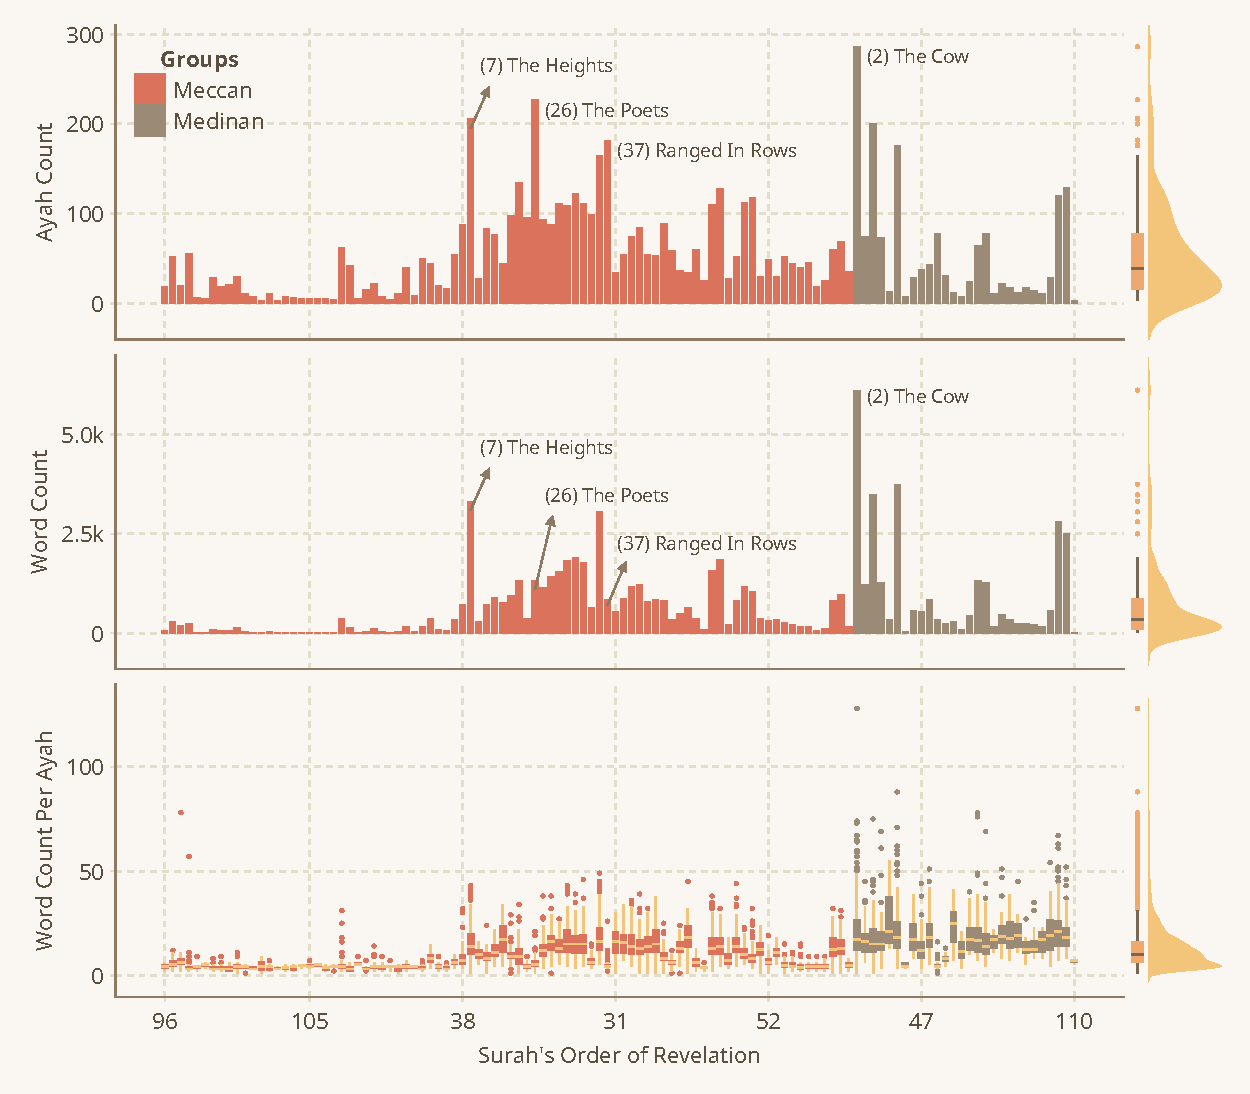
\includegraphics[width=\textwidth]{img/plot2.pdf}
    \caption{Statistics of the words and \arb[trans]{ayAt} \arb{ayAt} (verses) of the Qur'\=an according to revelation order}
    \label{fig:result_ayah_word_count_rev_order}
\end{figure}

\begin{figure}[!t]
    \centering
    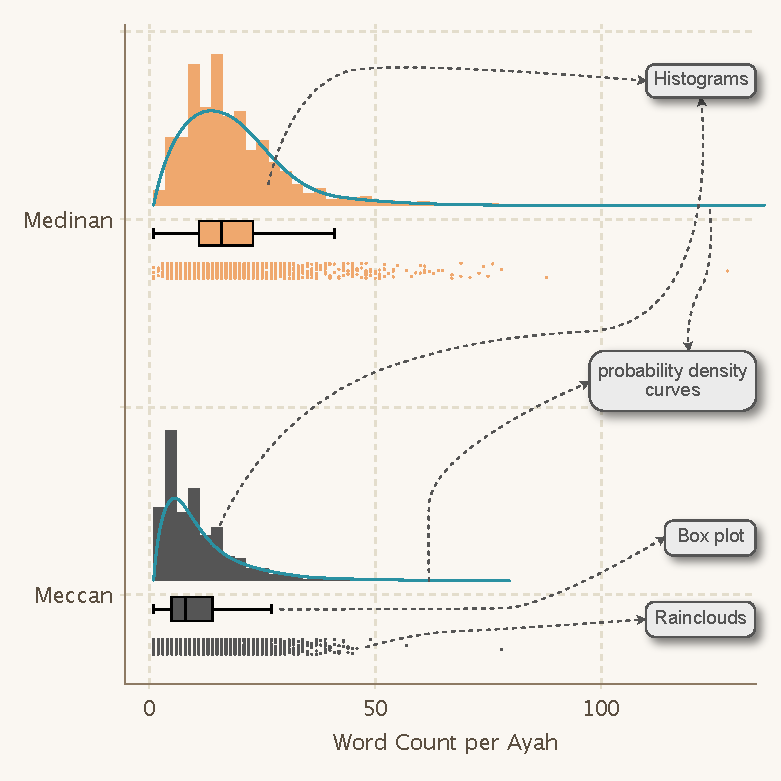
\includegraphics[width=\textwidth]{img/plot3.pdf}
    \caption{Distribution of Meccan and Medinan \arb[trans]{sUwar} \arb{sUwar}}
    \label{fig:result_meccan_medinan_dist}
\end{figure}

\begin{table}
    \caption{Descriptive statistics of the \arb[trans]{ayAt} \arb{ayAt} counts and the counts of its words}
    \label{tbl:desc_stats}
    \begin{tabularx}{\textwidth}[!h]{XXXX}
        \toprule
        Count Data&Mean&Median&Std. Deviation\\
        \midrule
        Ayahs&54.70&39&53.21\\
        Words&679.20&344&931.18\\
        Words per Ayah&10.27&8.23&6.35\\
        \bottomrule
    \end{tabularx}
\end{table}
\subsection{Comparison to Sinai's Inner-Chronology}
The work of \citeA{sinai2020oqs} investigated the same statistical distributions as in the previous section, but has focused from a non-traditionalist view by not basing on the \arb[trans]{'asbAb 'alnuzUl} \arb{'asbAb 'alnuzUl}, and instead mainly on the Qur'\=an's text itself using a transliteration data from Prof. Hans Zirker. The said data is not exactly the same as the one used in here, nor it is publicly verified as the one (Quranic Arabic Corpus and the Tanzil data) used in this study. Nonetheless, if indeed the said transliteration is exactly the same as the one used here once decoded to its Arabic form, the result should more or less be the same. However, while the preprocessing done by \citeA{sinai2020oqs} was not done in the analyses of the previous section, the result of the distributions should not deviate much. In the said study of \citeA{sinai2020oqs}, the findings suggest that there is inner-chronology of the Qur'\=an. This was concluded by the said author by looking at the mean verse length, which is more or less similar to the median verse length indicator used in boxplots of the third and fourth plots of Figures \ref{fig:result_ayah_word_count} and \ref{fig:result_ayah_word_count_rev_order}. Indeed, median is a better metric than mean in this case due to outlier counts seen in the boxplots in Figures \ref{fig:result_ayah_word_count} and \ref{fig:result_ayah_word_count_rev_order}. It is surprising though that he considered those with significant variance or coefficient variations (meaning those \arb[trans]{suwar} \arb{suwar} with very varied number of characters per \arb[trans]{ayAt} \arb{ayAt}) as possible later insertion to the Qur'\=an upon his closer inspection. It may sound polemic to disregard his findings or to attack it, but to be fair to Muslim traditionalists that to believe in such claim requires solid evidence from extant manuscripts and not just from someone's own interpretation of the statistics or literary styles of the \arb[trans]{ayAt} \arb{ayAt}. Indeed, the findings of Prof. Sina's can be categorized as \textit{theories} as it does not have supporting manuscripts that shows one. It may also be difficult to prove so as all Qur'\=anic extant manuscripts are consistent with the current one, including the controversial Sana'a Palimpest, where also Prof. Sinai was fair to admit in his own book \cite{sinai2017} that the said texts have. 

Furthermore, while it is healthy for the advancement of any studies including Qur'\=anic studies to have opposing views. For the case of \citeA{sinai2020oqs}, the premise of not considering \arb[trans]{'asbAb 'alnuzUl} \arb{'asbAb 'alnuzUl} shows a different structure as discussed in the preceding section.
\section{Morphological Analysis}\label{sec:ch4_morphological_analysis}
The second statistical analysis is to analyze the morphological features of the Qur'\=an. There are several ways to do this, and the easiest one is to find a particular word and study its morphologies. This will be the goal of this section, and the important word to study is the name of God in the Qur'\=an and that is \arb[trans]{'l-l_ah} \arb{'l-l_ah}. The root of this word is the \arb[trans]{Alh} \arb[novoc]{Alh}, and thus the morphologies of this root word will be studied and compared againts the \arb[trans]{'asbAb 'alnuzUl} \arb{'asbAb 'alnuzUl} or the 'occasions/circumstances of revelation.' Table \ref{tbl:result_Alh_morphologies} contains the complete list of morphologies of \arb[trans]{Alh} \arb[novoc]{Alh}. The first column in the said table lists the said morphologies, the second column lists its location in \arb[trans]{sUraT} \arb{sUraT} and \arb[trans]{'ayaT} \arb{'ayaT}, the third column lists the total number of \arb[trans]{'ayaT} \arb{'ayaT} that has the said morphology in the Qur'\=an, and the fourth column lists the percentage of \arb[trans]{'ayaT} \arb{'ayaT} whose \arb[trans]{'asbAb 'alnuzUl} \arb{'asbAb 'alnuzUl} is Mecca. The codes on how to generate this table in Julia using QuranTree.jl, Yunir.jl, and DataFrames.jl libraries are shown in Figure \ref{fig:result_Alh_morphologies}.

\begin{table}[!t]
    \begin{tabularx}{\textwidth}[!h]{cXcc}
        \toprule\\[-0.3cm]
        Morph. & Surah \& Ayah & Count & Meccan \% \\[0.2cm]
        \midrule\\[-0.4cm]
        \arb[fullvoc]{'l-l_ahi} & 1:1, 2:8, 2:23, $\cdots$, 104:6, 110:1, 110:2 & $710$ & 47\% \\[0.2cm]
        \arb[fullvoc]{llahi} & 1:2, 2:22, 2:98, $\cdots$, 71:13, 72:18, 82:19 & $122$ & 55\%\\[0.2cm]
        \arb[fullvoc]{'l-l_ahu} & 2:7, 2:10, 2:15, $\cdots$, 98:8, 112:1, 112:2 & $624$ & 39\% \\[0.2cm]
        \arb[fullvoc]{'l-l_aha} & 2:9, 2:26, 2:55, $\cdots$, 72:12, 96:14, 98:5 & $351$ & 30\% \\[0.2cm]
        \arb[fullvoc]{'il---a---_aha} & 2:133, 3:6, 6:106, $\cdots$, 45:23, 47:19, 73:9 & $17$ & 76\% \\[0.2cm]
        \arb[fullvoc]{'il---a---_ahu} & 2:163, 16:22, 18:110, $\cdots$ , 21:108, 29:46, 41:6 & $8$ & 88\% \\[0.2cm]
        \arb[fullvoc]{'il---a---_ahiN} & 3:62, 28:38, 38:65 & $3$ & 67\%\\[0.2cm]
        \arb[fullvoc]{|"'AlihaTaN} & 6:74, 18:15, 21:21, $\cdots$, 36:23, 37:86, 43:45 & $9$ & 100\% \\[0.2cm]
        \arb[fullvoc]{|"'Alihata} & 7:127, 21:36, 21:68, 71:23 & $4$ & 100\% \\[0.2cm]
        \arb[fullvoc]{'il---a---_ahaN} & 7:138, 18:14, 26:29 & $3$ & 100\%\\[0.2cm]
        \arb[fullvoc]{|"'Alihati} & 11:53, 11:54, 19:46, 25:42, 37:36, 37:91, 38:6, 46:22 & $8$ & 100\% \\[0.2cm]
        \arb[fullvoc]{|"'Alihatu} & 11:101 & $1$ & 100\% \\[0.2cm]
        \arb[fullvoc]{'il---a---_ahuN} & 14:52, 21:29, 43:84, 52:43 & $4$ & 100\% \\[0.2cm]
        \arb[fullvoc]{|"'AlihaTuN} & 17:42, 21:22, 21:43 & $3$ & 100\% \\[0.2cm]
        \arb[fullvoc]{'il---a---_ahi} & 20:97, 40:37, 114:3 & $3$ & 100\% \\[0.2cm]
        \arb[fullvoc]{--|"'Alihati}& 21:59, 21:62 & $2$ & 100\%\\[0.2cm]
        \arb[fullvoc]{|"'il---a---_ahuN} & 27:60, 27:61, 27:62, 27:63, 27:64 & $5$ & 100\% \\[0.2cm]
        \arb[fullvoc]{|"'AlihaTa} & 38:5 & $1$ & 100\% \\[0.2cm]
        \arb[fullvoc]{'alihatu} & 43:58 & $1$ & 100\% \\[0.2cm]
        \bottomrule
    \end{tabularx}
    \caption{Morphologies of \arb[novoc]{Alh} in the Qur'\=an}
    \label{tbl:result_Alh_morphologies}
\end{table}

The codes in Figure \ref{fig:result_Alh_morphologies} defines a Julia function called \verb|get_morphologies| from lines 5 to 25. The body of this function contains logics for extracting the morphologies of a given root word. At a high level, the logics has the following flow: it reads the morphological features of the root word \arb[novoc]{Alh}, then it lists down the chapter and verses containing this root word, and then compute the total number of \arb[trans]{AyAt} \arb{AyAt} that contain the given morphology of the given root word. Finally, it returns the output in tabular form that is presented in Table \ref{tbl:result_Alh_morphologies}. The defined \verb|get_morphologies| function can then be used to generate similar tables from other root words without rewriting those codes in lines 5 to 25 of Figure \ref{fig:result_Alh_morphologies}. Indeed, this is the beauty of programming, it can automate the manual process. For example, to generate similar table for the morphology of \arb{r.hm}, the code is as simple as shown in Figure \ref{fig:result_rHm_morphologies}, which shows only the first five morphologies of \arb{r.hm}.

\begin{figure}[!t]
    \centering
    \includegraphics[width=\textwidth]{img/morphologies_Alh.png}
    \caption{Julia code for generating Table \ref{tbl:result_Alh_morphologies}}
    \label{fig:result_Alh_morphologies}
\end{figure}

\begin{figure}[!t]
    \centering
    \includegraphics[width=\textwidth]{img/morphologies_rHm.png}
    \caption{Julia code for generating morphologies of \arb[novoc]{r.hm}}
    \label{fig:result_rHm_morphologies}
\end{figure}

From the result it can be observed that those these morphologies are purely under Meccan: \arb[trans]{'alihatu}  \arb[fullvoc]{'alihatu} - a masculine plural noun in nominative case (\textit{see} Figure \ref{fig:result_mfeat_43_58} for the codes on how to get these details in QuranTree.jl); \arb[trans]{|"'AlihaTa} \arb[fullvoc]{|"'AlihaTa} - a masculine plural noun in accusative case; \arb[trans]{|"'il---a---_ahuN} \arb[fullvoc]{|"'il---a---_ahuN} - a masculine singular noun in indefinite state and nominative case; \arb[trans]{--|"'Alihati} \arb[fullvoc]{--|"'Alihati} - a masculine plural noun in genitive case; \arb[trans]{'il---a---_ahi} \arb[fullvoc]{'il---a---_ahi} - a masculine singular noun in genitive case; \arb[trans]{|"'AlihaTuN} \arb[fullvoc]{|"'AlihaTuN} - a masculine plural noun in indefinite state and nominative case; \arb[trans]{'il---a---_ahuN} \arb[fullvoc]{'il---a---_ahuN} - similar to \arb[trans]{|"'il---a---_ahuN} \arb[fullvoc]{|"'il---a---_ahuN} with slightly different morphology; \arb[trans]{|"'Alihatu} \arb[fullvoc]{|"'Alihatu} - a masculine plural noun in nominative case; \arb[trans]{|"'Alihati} \arb[fullvoc]{|"'Alihati} - a masculine plural noun in genitive case; \arb[trans]{'il---a---_ahaN} \arb[fullvoc]{'il---a---_ahaN} - a masculine singular noun in indefinite state and accusative case; \arb[trans]{|"'Alihata} \arb[fullvoc]{|"'Alihata} - a masculine plural noun in accusative state, \arb[trans]{|"'AlihaTaN} \arb[fullvoc]{|"'AlihaTaN} - a masculine plural noun in indefinite state and accusative case.

\begin{figure}[!t]
    \centering
    \includegraphics[width=\textwidth]{img/mfeat_43_58.png}
    \caption{Julia code for describing morphological features of \arb[trans]{'alihatu} \arb{'alihatu}}
    \label{fig:result_mfeat_43_58}
\end{figure}

The last column in Table \ref{tbl:result_Alh_morphologies} contains the percentages of the Meccan \arb[trans]{AyAt} \arb{AyAt}, therefore among the \arb[trans]{AyAt} \arb{AyAt} that contain the morphologies of \arb[trans]{'l-l_ahi} \arb[fullvoc]{'l-l_ahi} is that 47\% of those are Meccan. This column was generated by the code in Figure \ref{fig:result_meccan_ratio}.

\begin{figure}[!t]
    \centering
    \includegraphics[width=\textwidth]{img/meccan_ratio.png}
    \caption{Julia code for generating last column of Table \ref{tbl:result_meccan_ratio}}
    \label{fig:result_meccan_ratio}
\end{figure}

Sample \arb[trans]{AyAt} \arb{AyAt} are given for Q43:59, Q21:59, and Q2:23. The first \arb[trans]{'ayaT} \arb{'ayaT} contains the only morphology for \arb[trans]{'alihatu} \arb[fullvoc]{'alihatu} in the Qur'\=an, which is highlighted in red. The context of this \arb[trans]{'ayaT} \arb{'ayaT} is that it the \textit{gods} (\arb[trans]{'alihatu} \arb[fullvoc]{'alihatu}) referred here are the dieties worshipped by the disbelievers. The one they cited here as \textit{him} is given in the previous  \arb[trans]{'ayaT} \arb{'ayaT} as Jesus \txarb{\fontspec{Scheherazade New} ﵇}, the son of Mary \txarb{\fontspec{Scheherazade New} ﵍}. 

\begin{bottomtitledframe}{Q43:58}
    \begin{center}
        \begin{arab}[fullvoc]
            min ((sUraTu 'l-zuxrufi)): waqAlUA |"'a\arbcolor[red]{'a_alihatu}nA xayruN 'am huwa mA .darabUhu laka 'illA jadalA bal hum qawmun xA.simUn
        \end{arab}
        \begin{arab}[trans]
            min ((sUraTu 'l-zuxrufi)): waqAlUA |"'a\arbcolor[red]{'a_alihatu}nA xayruN 'am huwa mA .darabUhu laka 'illA jadalA bal hum qawmun xA.simUn
        \end{arab}
    \end{center}
    From Surah \textit{Ornaments of Gold}: saying, 'Are our \textcolor{red}{gods} better or him?' --- they cite him only to challenge you: they are a contentious people ---
\end{bottomtitledframe}

The next Meccan \arb[trans]{'ayaT} \arb{'ayaT} is Q21:59, which contain the morphology for \arb[trans]{--|"'Alihati} \arb[fullvoc]{--|"'Alihati}, which refers to \textit{gods} or \textit{deities} of the disbelievers. In this \arb[trans]{'ayaT} \arb{'ayaT} the question is coming from disbelievers during the time of Abraham \txarb{\fontspec{Scheherazade New} ﵇}, after he destroyed the idols worshipped by his father and the disbelievers. Indeed, the not so common morphologies for \arb[novoc]{alh} refer to false gods and dieties and not to the true God that the Qur'\=an refers to. 

\begin{bottomtitledframe}{Q21:59}
    \begin{center}
        \begin{arab}[fullvoc]
            min ((sUraTu 'l-'anbiyA'i)): waqAlUA man fa`ala ha_a_dA bi\arbcolor[red]{--|"'Alihati}n'A 'innahu lamina 'l-.za_alimIna
        \end{arab}
        \begin{arab}[trans]
            min ((sUraTu 'l-'anbiyA'i)): waqAlUA man fa`ala ha_a_dA bi\arbcolor[red]{--|"'Alihati}n'A 'innahu lamina 'l-.za_alimIna
        \end{arab}
    \end{center}
    From Surah \textit{The Prophets}: They said, 'Who has done this to our \textcolor{red}{gods}? How wicket he must be!
\end{bottomtitledframe}

Finally, the example for the use of \arb[novoc]{alh} morphology to refer to the true God in the Qur'\=an is given in Q2:23, for \arb[trans]{'l-lahi} \arb[fullvoc]{'l-lahi}. Here the context is the challenge of Allah or God to the disbelievers to produce a single \textit{s\=urah} \arb{sUraT} or chapter like that in the Qur'\=an. This is indeed a challenge that is still valid until today, and no one has ever produced a single \textit{s\=urah} \arb{sUraT} like the Qur'\=an. If there was one, it should have been published in a reputable journal addressing this challenge. The problem with producing this is that it should be with the same eloquence and beauty of the Qur'\=an. This is indeed a challenge that is still valid until today, and no one has ever produced a single \textit{s\=urah} \arb{sUraT} like the Qur'\=an. This is part of the \arb[trans]{'al-'i`jAzu 'l-qur`an} \arb{'al-'i`jAzu 'l-qur`an} or \textit{the inimitability of the Qur'\=an}, which is one of the main reasons why the Qur'\=an is considered to be a miracle by the Muslims.

\begin{bottomtitledframe}{Q2:23}
    \begin{center}
        \begin{arab}[fullvoc]
            min ((sUraTu 'l-baqaraTi)): wa-'in kuntum fI raybiN mmimmA nazzalnA `alY_a `abdinA fa'tUA bisUraTiN mmin mmi_tlihi wa-"ad`UA ^suhada'A'akum mmin dUni \arbcolor[red]{'l-lahi} 'in kuntum .sa--_a--diqIna
        \end{arab}
        \begin{arab}[trans]
            min ((sUraTu 'l-baqaraTi)): wa-'in kuntum fI raybiN mmimmA nazzalnA `alY_a `abdinA fa'tUA bisUraTiN mmin mmi_tlihi wa-"ad`UA ^suhada'A'akum mmin dUni \arbcolor[red]{'l-lahi} 'in kuntum .sa--_a--diqIna
        \end{arab}
    \end{center}
    From Surah \textit{The Cow}: If you have doubts about the revelation We have sent down to Our servant, then produce a single surah like it --- enlist whatever supporters you have other than \textcolor{red}{God} --- if you truly [think you can].
\end{bottomtitledframe}

The results shown in Table \ref{tbl:result_Alh_morphologies} found several verses for the common morphologies of \arb[novoc]{alh}, while those rare ones have been found by the codes in Figure \ref{fig:result_Alh_morphologies}. In fact, the whole results in Table \ref{tbl:result_Alh_morphologies} were generated in under 5 seconds and few lines of codes from Figure \ref{fig:result_Alh_morphologies} and \ref{fig:result_meccan_ratio}. Had it been done manually, it would have taken days, weeks or even months. Plus the final results will likely have human errors, or at least it will need another person to verify the results, which too will take time. This is the main advantage of programming as it can automate such process with great accuracy, so long as the codes are accurate. Generating new morphologies for any given root can be done in just one line of code as in the first line of code in Figure \ref{fig:result_rHm_morphologies}.

% \begin{bottomtitledframe}{Q43:58}
%    Hello!
% \end{bottomtitledframe}



\section{Thematic Analysis}\label{sec:result_thematic_analysis}
From previous section, it was concluded that those morphologies that are unique to Meccan \arb[trans]{sUwar} \arb{sUwar} are considered to refer to false gods or deities worshipped by the disbelievers. Whereas those with common morphologies are considered to refer to the true God. Sample \arb[trans]{sUwar} \arb{sUwar} were given above for three \arb[trans]{ayaT} \arb{ayaT}, but it would be better to also understand the themes of \arb[trans]{AyAt} \arb{AyAt} for other morphologies, especially those that are common. However, doing this manually would be very tedious and time consuming, since the first morphology, \arb[trans]{'l-lahi} \arb[fullvoc]{'l-lahi}, contain 710 \arb[trans]{AyAt} \arb{AyAt}. Trying to summarize this manually would take so much time, and will also be prone to human error. How to automate then?

In Statistics and Machine Learning, there are techniques to do this mathematically. Among the basic method is what is called Latent Dirichlet Allocation (LDA), an algorithm that can produce keywords as topics from a given text. The algorithm is based on the idea that each document is a mixture of topics, and each topic is a mixture of words. The algorithm works by assigning each word in the document to a topic, and then updating the topic assignments based on the words assigned to each topic. This process is repeated until the topic assignments converge. The result is a set of topics, each represented by a set of words, that can be used to summarize the document. LDA has been effective for topic modeling and has been widely used in various applications, including text classification, information retrieval, and document clustering.

Another approach to topic modeling is using the BERT (Bidirectional Encoder Representations from Transformers) model, in layman's term, it is an artificial intelligence model that can understand the meaning of words in a sentence by looking at the context of the words around it. The idea is that BERT can generate a numerical representation of a word or a sentence, which can then be used to find similar words or sentences. Since it can be used to find similar words, it therefore can be used to find themes --- which groups similar words. This concept is called BERTopic. 

The third approach to topic modeling or thematic clustering is to use Generative Pre-trained Transformer (GPT) model. The idea is that GPT can generate a summary of a given text, and this summary can be used to find the themes of the text. This approach is similar to LDA, but it uses a different algorithm to generate the summary. The advantage of using GPT is that it can generate a more accurate summary than LDA, and it can also be used to generate summaries for longer texts. For many readers, ChatGPT is the most popular AI model. Indeed, this is the GPT model referred here. 

Among the three approaches mentioned, the third one is the best for the study as it can do everything the first two approaches do, but with human-readable summary and many GPT models have been trained on Qur'\=an data. There are many open-sourced GPT models that can be used, but those commercialized one are more accurate, such as the ChatGPT or the ClaudeAI. For this study, Claude 3.7 Sonnet GPT model is used.

\begin{listing2}[!t]
    \centering
    \includegraphics[width=\textwidth]{img/ayah_morph_extract.png}
    \caption{Julia code for generating last column of Table \ref{tbl:result_meccan_ratio}}
    \label{fig:result_thematic_analysis}
\end{listing2}

% \begin{table}[!h]
%     \begin{tabularx}{\textwidth}[!h]{cXcc}
%         \toprule\\[-0.3cm]
%         Morph. & Surah \& Ayah & Count & Meccan \% \\[0.2cm]
%         \midrule\\[-0.4cm]
%         \arb[fullvoc]{'l-l_ahi} & Divine Unity \& Singularity (Tawhid) [6:164, 28:88, 2:163]; Faith \& Belief (Iman) [49:15, 65:11]; Divine Guidance \& Revelation [2:2, 5:48]; Prophet \& Messengers [2:136, 48:29]; The Day of Judgement \& Afterlife [2:281, 68:34]; Moral \& Ethical Teachings [16:90, 5:1]; Stories of Previous Nations [47:10]; Relationship Between Allah \& Creation [50:16, 51:56]; Rules \& Legislation [62:9, 4:2]; Struggle \& Perseverance [22:78, 2:155] & $710$ & 47\% \\[0.2cm]
%         \arb[fullvoc]{llahi} & Divine Sovereignty \& Ownership [2:284, 3:109, 3:129]; Divine Attributes [4:170, 31:26, 4:139, 9:91]; Creator \& Sustainer [6:1, 35:1]; Purpose of Worship [53:62, 22:31]; Divine Judgement \& Authority [22:56, 24:64, 3:129]; Gratitude \& Praise [1:2, 6:1, 34:1, 35:1]; Divine Will \& Power [14:4, 3:129]; Submission to Allah [2:112, 4:125] & $122$ & 55\%\\[0.2cm]
%         \arb[fullvoc]{'l-l_ahu} & Divine Unity \& Singularity (Tawhid) [112:1, 2:255, 2:116, 10:68]; Divine Sovereignty \& Power [7:54, 10:3]; Divine Knowledge [3:29, 9:94]; Divine Justice [40:20, 3:57]; Divine Guidance [2:213, 24:46, 57:25]; Divine Will \& Decree [14:27, 5:48]; Divine Names \& Attributes [59:24, 24:35]; Relationship with Believers [98:8]; Divine Creation \& Sustenance [23:14, 7:54]  & $624$ & 39\% \\[0.2cm]
%         \arb[fullvoc]{'l-l_aha} & Divine Unity \& Singularity (Tawhid) [7:59, 19:36, 98:5]; Divine Attributes [49:16, 9:5, 2:284]; Obedience to Allah \& His Messenger [4:59, 64:12, 48:17]; Piety \& God Conciousness [3:102, 2:194, 8:25]; Reward \& Punishment [47:12, 40:17, 22:14]; Prayer, Charity, \& Righteous Deeds [98:5]; Stories of Prophets \& Past Nations [11:50, 11:61]; Faith \& Belief [49:10]; Justice \& Fairness [16:90] & $351$ & 30\% \\[0.2cm]
%         \arb[fullvoc]{'il---a---_aha} & 2:133, 3:6, 6:106, $\cdots$, 45:23, 47:19, 73:9 & $17$ & 76\% \\[0.2cm]
%         \arb[fullvoc]{'il---a---_ahu} & 2:163, 16:22, 18:110, $\cdots$ , 21:108, 29:46, 41:6 & $8$ & 88\% \\[0.2cm]
%         \arb[fullvoc]{'il---a---_ahiN} & 3:62, 28:38, 38:65 & $3$ & 67\%\\[0.2cm]
%         \arb[fullvoc]{|"'AlihaTaN} & 6:74, 18:15, 21:21, $\cdots$, 36:23, 37:86, 43:45 & $9$ & 100\% \\[0.2cm]
%         \arb[fullvoc]{|"'Alihata} & 7:127, 21:36, 21:68, 71:23 & $4$ & 100\% \\[0.2cm]
%         \arb[fullvoc]{'il---a---_ahaN} & 7:138, 18:14, 26:29 & $3$ & 100\%\\[0.2cm]
%         \arb[fullvoc]{|"'Alihati} & 11:53, 11:54, 19:46, 25:42, 37:36, 37:91, 38:6, 46:22 & $8$ & 100\% \\[0.2cm]
%         \arb[fullvoc]{|"'Alihatu} & 11:101 & $1$ & 100\% \\[0.2cm]
%         \arb[fullvoc]{'il---a---_ahuN} & 14:52, 21:29, 43:84, 52:43 & $4$ & 100\% \\[0.2cm]
%         \arb[fullvoc]{|"'AlihaTuN} & 17:42, 21:22, 21:43 & $3$ & 100\% \\[0.2cm]
%         \arb[fullvoc]{'il---a---_ahi} & 20:97, 40:37, 114:3 & $3$ & 100\% \\[0.2cm]
%         \arb[fullvoc]{--|"'Alihati}& 21:59, 21:62 & $2$ & 100\%\\[0.2cm]
%         \arb[fullvoc]{|"'il---a---_ahuN} & 27:60, 27:61, 27:62, 27:63, 27:64 & $5$ & 100\% \\[0.2cm]
%         \arb[fullvoc]{|"'AlihaTa} & 38:5 & $1$ & 100\% \\[0.2cm]
%         \arb[fullvoc]{'alihatu} & 43:58 & $1$ & 100\% \\[0.2cm]
%         \bottomrule
%     \end{tabularx}
%     \caption{Morphologies of \arb[novoc]{Alh} in the Qur'\=an}
%     \label{tbl:result_Alh_morphologies_theme}
% \end{table}

\section{Rhythmic Analysis}\label{sec:result_rhythmic_analysis}
As already emphasized in repeatedly in this paper is that the Qur'\=an rhymes. This rhythm is not only important for the recitation of the Qur'\=an, but it also plays a significant role in the meaning and interpretation of the text. The rhythm of the Qur'\=an is created by the use of various literary devices, such as alliteration and assonance, which help with the rhythm whose dynamics also gives recitations with sounds whose transition yields different emotions. A good example of this is the \arb[trans]{sUraTu 'l-qAri`ati} \arb{sUraTu 'l-qAri`ati} shown in Table \ref{tbl:surah_alqariah}.

\begin{table}[!h]
    \caption{The verses or \arb[trans]{'AyAt} \arb{'AyAt} of \arb[trans]{sUraTu 'l-qAri`ati} \arb{sUraTu 'l-qAri`ati}}
    \begin{tabularx}{\textwidth}{cXr}
        \toprule
        \textbf{No.}&\textbf{Transliteration \& }&\textbf{Verses} or \arb[trans]{'AyAt} \arb{'AyAt}\\
        &\textbf{Translation}&\\
        \midrule
        
        &\arb[trans]{bismi 'l-lahi 'l-ra.hm_ani 'l-ra\arbcolor[red]{hIm}\arbcolor[gray]{i}}&
        \multirow{2}{*}{\arb[fullvoc]{bismi 'l-l_ahi 'l-ra.hm_ani 'l-ra\arbcolor[red]{hIm"}\arbcolor[gray]{.i}}}\\[0.1cm]
        &In the name of God, the Lord of Mercy, the Giver of Mercy!&\\[1cm]

        1&\arb[trans]{'l-qAri\arbcolor[red]{`a}\arbcolor[gray]{Tu}};&
        \multirow{2}{*}{\arb[fullvoc]{'l-q--Ari\arbcolor[red]{`a}\arbcolor[gray]{Tu}}}\\[0.1cm]
        &The Crashing Blow!&\\[0.5cm]

        2&\arb[trans]{mA 'l-qAri\arbcolor[red]{`a}\arbcolor[gray]{Tu}}&
        \multirow{2}{*}{\arb[fullvoc]{mA 'l-q--Ari\arbcolor[red]{`a}\arbcolor[gray]{Tu}}}\\[0.1cm]
        &What is the Crashing Blow?&\\[0.5cm]
        
        3&\arb[trans]{wama'A 'adra--_a--ka mA 'l-q--Ari\arbcolor[red]{`a}\arbcolor[gray]{Tu}}&
        \multirow{2}{*}{\arb[fullvoc]{wama'A 'adra--_a--ka mA 'l-qAri\arbcolor[red]{`a}\arbcolor[gray]{Tu}}}\\[0.1cm]
        &What will explain to you what the Crashing Blow is?&\\[1cm]

        4&\arb[trans]{yawma y--a--kUnu 'l-nAsu ka-'l-farA^si 'l-mab\arbcolor[red]{_tU_t"}\arbcolor[gray]{.i}}&
        \multirow{2}{*}{\arb[fullvoc]{yawma y--a--kUnu 'l-nAsu ka-'l-farA^si 'l-mab\arbcolor[red]{_tU_t"}\arbcolor[gray]{.i}}}\\[0.1cm]
        &On a Day when people will be like scattered moths&\\[1cm]

        5&\arb[trans]{fatakUnu 'l-jibAlu ka-'l-`ihni 'l-man\arbcolor[red]{fU^s"}\arbcolor[gray]{.i}}&
        \multirow{2}{*}{\arb[fullvoc]{fatakUnu 'l-jibAlu ka-'l-`ihni 'l-man\arbcolor[red]{fU^s"}\arbcolor[gray]{.i}}}\\[0.1cm]
        &and the mountains like tufts of wool,&\\[0.5cm]

        6&\arb[trans]{fa'ammA man _taqulat mawa_azI\arbcolor[red]{nuh"}\arbcolor[gray]{.u}}&
        \multirow{2}{*}{\arb[fullvoc]{fa--'ammA man _ta--qulat mawa--_azI\arbcolor[red]{nuh"}\arbcolor[gray]{.u}}}\\[0.1cm]
        &the ones whose good deeds are heavy on the scales&\\[1cm]

        7&\arb[trans]{fahuwa fiY `I^saTiN rA.di\arbcolor[red]{yaT"}\arbcolor[gray]{.iN}}&
        \multirow{2}{*}{\arb[fullvoc]{fahuwa fiY `I^saTiN rA.di\arbcolor[red]{yaT"}\arbcolor[gray]{iN}}}\\[0.1cm]
        &will have a pleasant life,&\\[0.5cm]

        8&\arb[trans]{wa'ammA man xaffat mawa--_azI\arbcolor[red]{nuh"}\arbcolor[gray]{.u}}&
        \multirow{2}{*}{\arb[fullvoc]{wa'ammA man xaffat mawa--_azI\arbcolor[red]{nuh"}\arbcolor[gray]{.u}}}\\[0.1cm]
        &but the one whose good deeds are light&\\[0.5cm]

        9&\arb[trans]{fa-'ummuhu hAwi\arbcolor[red]{yaT"}\arbcolor[gray]{uN}}&
        \multirow{2}{*}{\arb[fullvoc]{fa-'ummuhu hAwi\arbcolor[red]{yaT"}\arbcolor[gray]{uN}}}\\[0.1cm]
        &will have the Bottomless Pit for his home--&\\[0.5cm]


        10&\arb[trans]{wama'A 'adra--_a--ka mA hi\arbcolor[red]{yah}}&
        \multirow{2}{*}{\arb[fullvoc]{wama'A 'adra--_a--ka mA hi\arbcolor[red]{yah"}}}\\[0.1cm]
        &what will explain to you what that is?---&\\[0.5cm]

        11&\arb[trans]{nAruN .hAmi\arbcolor[red]{yaT"}\arbcolor[gray]{.u}}&
        \multirow{2}{*}{\arb[fullvoc]{nAruN .hAmi\arbcolor[red]{yaT"}\arbcolor[gray]{.u}}}\\[0.1cm]
        &a blazing fire.&\\[0.1cm]
        \bottomrule

    \end{tabularx}
    \label{tbl:surah_alqariah}
\end{table}

The first three \arb[trans]{'AyAt} \arb{'AyAt}, which contain repetition and questioning with the word \arb[trans]{'l-qAri\arbcolor[red]{`a}\arbcolor[gray]{Tu}} \arb[fullvoc]{'l-qAri\arbcolor[red]{`a}\arbcolor[gray]{Tu}}. Note that, the red color indicates that this is the last recited syllable, while the gray color means it is silent and is not recited when reciting the Qur'\=an. The word \arb[trans]{'l-qAri`aTu} \arb[fullvoc]{'l-qAri`aTu} creates a striking, percussive effect with its hard consonant sounds (especially the \textit{qaf} letter \arb{q} and the \textit{ayn} letter \arb{`--}). This phonetic quality mimics a knocking or crashing sound, which aligns perfectly with the meaning of "The Crashing Blow." The short, staccato phrases build tension and create a sense of urgency and alarm appropriate for introducing the Day of Judgment. 

The letter \textit{qaf} (\arb{q}) in \arb[trans]{'l-qAri`aTu} \arb[fullvoc]{'l-qAri`aTu} provides the most prominent staccato effect. The qaf is a strong, emphatic consonant pronounced from deep in the throat with a distinctive "popping" quality that creates a percussive sound when articulated properly.The letter \textit{ayn} (\arb{`--}) in \arb[trans]{'l-qAri`aTu} \arb[fullvoc]{'l-qAri`aTu} also contributes to the staccato effect. The \textit{ayn} is a guttural stop consonant that requires a distinct articulation, creating another percussive element. The letter \textit{hamza} (\arb{|"'}) in \arb[trans]{ma'A 'adra--_a--ka} \arb{ma'A 'adra--_a--ka} produces a glottal stop that adds to the choppy, staccato rhythm. The \textit{tah marbuta} (\arb{--T}) at the end of \arb[trans]{'l-qAri`aTu} \arb[fullvoc]{'l-qAri`aTu} creates a stopping point that enhances the abrupt quality of each phrase.

As the \arb[trans]{sUraT} \arb{sUraT} moves to verses or \arb[trans]{'AyAt} \arb{'AyAt} 4 to 5, the rhythm extends into longer phrases describing scattered moths and tufts of wool. Here, the \arb[trans]{sUraT} \arb{sUraT} provides the first descriptive details of this event, maintaining the same topic but with a slightly different rhythm as it shifts \textit{from questioning to description}. In these \arb[trans]{'AyAt} \arb{'AyAt}, the Qur'\=an uses words with \textit{flowing sounds} that phonetically evoke the visual imagery of things being scattered and fluffed apart, mirroring the chaos described. Words like \arb[trans]{y--a--k"\arbcolor[red]{U}nu} \arb[fullvoc]{y--a--k"\arbcolor[red]{U}nu} have the long vowel \arb[trans]{U} that extends the sound, creating a flowing effect. Further, the sibilant consonant \textit{shin} \arb{^s} (transliterated as \arb[trans]{^s}) for "sh" sound in \arb[trans]{ka-'l-farA\arbcolor[red]{^si}} \arb[fullvoc]{ka-'l-farA\arbcolor[red]{^si}} and in \arb[trans]{ka-'l-`ihni 'l-man\arbcolor[red]{fU^s"}\arbcolor[gray]{.i}} \arb[fullvoc]{ka-'l-`ihni 'l-man\arbcolor[red]{fU^s"}\arbcolor[gray]{.i}} creates a continuous airflow rather than a stopped sound. This is also true with the \textit{tha} \arb{_t} (transliterated as \arb[trans]{_t}) for "th" sound in \arb[trans]{'l-mab\arbcolor[red]{_tU_t"}\arbcolor[gray]{.i}} \arb{'l-mab\arbcolor[red]{_tU_t"}\arbcolor[gray]{.i}}. The Nasal sounds, "n" and "m", in words like \arb[trans]{'l-\arbcolor[red]{man}fU^si} \arb[fullvoc]{'l-\arbcolor[red]{man}fU^si} create resonance that extends the sound. Further, \arb[trans]{'AyAt} \arb{'AyAt} 4 to 5 use longer, more connected phrasal structures compared to the choppy opening verses in \arb[trans]{'AyAt} \arb{'AyAt} 1 to 3.

The first major topical and rhythmic shift occurs at verse 6, where the focus changes from describing the cataclysmic event itself to explaining the judgment of individuals. The shift in sound starts with the first word in \arb[trans]{'ayaT} \arb{'ayaT} 6, \arb[trans]{fa'ammA} \arb[fullvoc]{fa'ammA}, which introduces the letter \textit{mim} \arb{m} (transliterated as \arb[trans]{m}) for "m" sound. This creates a new rhythmic pattern where the "m" sound is repeated in the verses creating a humming, resonant quality. The rhythm becomes more measured and deliberate, this is because of the balanced phrasing, \arb[trans]{fa'ammA man _taqulat} \arb[fullvoc]{fa'ammA man _taqulat} in \arb[trans]{'ayaT} \arb{'ayaT} 6 and  \arb[trans]{wa'ammA man xaffat} \arb[fullvoc]{wa'ammA man xaffat} in \arb[trans]{'ayaT} \arb{'ayaT} 8, have both almost the same number of syllables, with verse 7 syllables for \arb[trans]{'ayaT} \arb{'ayaT} 6 and 6 syllables for \arb[trans]{'ayaT} \arb{'ayaT} 8. Then both verse 6 and 8 ends with the same word, \arb[trans]{mawa--_azI\arbcolor[red]{nuh"}\arbcolor[gray]{.u}} \arb[fullvoc]{mawa--_azI\arbcolor[red]{nuh"}\arbcolor[gray]{.u}}. Further, \arb[trans]{'ayaT} \arb{'ayaT} 6 to 9 form pairs, with \arb[trans]{'ayaT} \arb{'ayaT} 6 to 7 describe one outcome (heavy scales $\rightarrow$ pleasant life), and \arb[trans]{'ayaT} \arb{'ayaT} 8 to 9 describe the contrasting outcome (light scales $\rightarrow$ abyss). The balanced structure creates a rhythmic swinging sensation that mimics the weighing of scales. The swinging is based on the transition from \arb[trans]{'ayaT} \arb{'ayaT} 7 back to the sound of \arb[trans]{'ayaT} \arb{'ayaT} 6 in \arb[trans]{'ayaT} \arb{'ayaT} 8. 

The final shift in \arb[trans]{sUraTu 'l-qAri`ati} \arb{sUraTu 'l-qAri`ati} occurs in verses 10 to 11. In these \arb[trans]{'ayaT} \arb{'ayaT}, the \arb[trans]{sUraT} \arb{sUraT} returns to a questioning style reminiscent of the opening \arb[trans]{'AyAt} \arb{'AyAt}\newline but with a different purpose, that instead of introducing \textit{the Crashing Blow} in \arb[trans]{'AyAt} \arb{'AyAt}, the questionning style refers back to \arb[trans]{hAwi\arbcolor[red]{yaT"}\arbcolor[gray]{uN}} \arb[fullvoc]{hAwi\arbcolor[red]{yaT"}\arbcolor[gray]{uN}} the \textit{Bottomless Pit} mentioned in verse 9, not to \arb[trans]{'l-qAri\arbcolor[red]{`a}\arbcolor[gray]{Tu}} \arb[fullvoc]{'l-qAri\arbcolor[red]{`a}\arbcolor[gray]{Tu}} mention in \arb[trans]{'AyAt} \arb{'AyAt} 1 to 3. The \arb[trans]{sUraT} \arb{sUraT} concludes with the revelation of the intense fire. In terms of sound, verse 10 ends with the shortened, abrupt \arb[trans]{hi\arbcolor[red]{yah}} \arb[fullvoc]{hi\arbcolor[red]{yah}} instead of the longer \arb[trans]{'l-qAri\arbcolor[red]{`a}\arbcolor[gray]{Tu}} \arb[fullvoc]{'l-qAri\arbcolor[red]{`a}\arbcolor[gray]{Tu}}. This creates a sudden stopping effect that heightens tension. Finally, verse 11 \arb[trans]{nAruN .hAmi\arbcolor[red]{yaT"}\arbcolor[gray]{.u}} \arb[fullvoc]{nAruN .hAmi\arbcolor[red]{yaT"}\arbcolor[gray]{.u}} is exceptionally brief and punchy compared to earlier descriptive verses, and uses a harsh consonant \arb[trans]{.h} which is a throat-scraping "h" sound in \arb[trans]{\arbcolor[red]{.h"}A\arbcolor[red]{m"}iyaT"\arbcolor[gray]{.u}} \arb[fullvoc]{\arbcolor[red]{.h"}A\arbcolor[red]{m"}iyaT"\arbcolor[gray]{.u}}, plus the emphatic "m" sound highlighted in red as well, delivering the ultimate revelation with emphatic force.

This rhythmic progression isn't merely decorative but integral to the \arb[trans]{sUraT}'s \arb{sUraT}\newline message, creating a complete sensory experience where sound reinforces meaning. The shift from chaotic disruption to measured judgment to final pronouncement helps listeners internalize the \arb[trans]{sUraT}'s \arb{sUraT} eschatological narrative about accountability and consequences.

The \arb[trans]{sUraT} \arb{sUraT} demonstrates how the Quranic text masterfully employs sound as a vehicle for meaning, where the rhythm itself becomes a form of exegesis - explaining and reinforcing the content through the physical experience of recitation and listening.

Before diving into the computational methods for analyzing these rhythms, another example showcasing a different rhythm is the \arb[trans]{sUraTu 'l-tIni} \arb{sUraTu 'l-tIni}. In this \arb[trans]{sUraT} \arb{sUraT}, there are 8 verses or \arb[trans]{'AyAt} \arb{'AyAt}. The first three can be grouped together as they form unique rhythm. The rhythm here is measured and ceremonial, with each \arb[trans]{'ayaT} \arb{'ayaT} beginning with the oath particle \arb[trans]{wa} \arb{wa} or \textit{by}. This creates a solemn, formal cadence that draws attention to these sacred symbols. 

As the \arb[trans]{sUraT} \arb{sUraT} moves to verses 4 to 6, the \arb[trans]{'AyAt} \arb{'AyAt}. The rhythm changes noticeably. The verses become longer and more complex, especially verse 6, which extends significantly compared to the earlier verses. The topic shifts dramatically from sacred symbols to human creation, fall, and salvation. The rhythm reflects this shift, becoming more narrative and expansive.

Finally, the last section shifts again in rhythm, becoming interrogative and direct. The verses are sharp and pointed, ending with rhetorical questions that demand reflection. The topic transforms into a challenge to the disbelievers, questioning their denial given the evidence previously presented.

\begin{table}[!h]
    \caption{The verses or \arb[trans]{'AyAt} \arb{'AyAt} of \arb[trans]{sUraTu 'l-tIni} \arb{sUraTu 'l-tIni}}
    \begin{tabularx}{\textwidth}{cXr}
        \toprule
        \textbf{No.}&\textbf{Transliteration \& }&\textbf{Verses} or \arb[trans]{'AyAt} \arb{'AyAt}\\
        &\textbf{Translation}&\\
        \midrule
        
        &\arb[trans]{bismi 'l-lahi 'l-ra.hm_ani 'l-ra\arbcolor[red]{hIm}\arbcolor[gray]{i}}&
        \multirow{2}{*}{\arb[fullvoc]{bismi 'l-l_ahi 'l-ra.hm_ani 'l-ra\arbcolor[red]{hIm"}\arbcolor[gray]{.i}}}\\[0.1cm]
        &In the name of God, the Lord of Mercy, the Giver of Mercy!&\\[1cm]

        1&\arb[trans]{wa-'l-tIni wa-'l-jay\arbcolor[red]{tUn"}\arbcolor[gray]{.i}};&
        \multirow{2}{*}{\arb[fullvoc]{wa-'l-tIni wa-'l-jay\arbcolor[red]{tUn"}\arbcolor[gray]{.i}}}\\[0.1cm]
        &By the fig, by the olive,&\\[0.5cm]

        2&\arb[trans]{wa.tUri sI\arbcolor[red]{nIn"}\arbcolor[gray]{.a}}&
        \multirow{2}{*}{\arb[fullvoc]{wa.tUri sI\arbcolor[red]{nIn"}\arbcolor[gray]{.a}}}\\[0.1cm]
        &by Mount Sinai,&\\[0.5cm]
        
        3&\arb[trans]{waha--_a_dA 'l-baladi 'l-'a\arbnull{mIni}\arbcolor[red]{mIn"}\arbcolor[gray]{.i}}&
        \multirow{2}{*}{\arb[fullvoc]{waha--_a_dA 'l-baladi 'l-'a\arbcolor[red]{mIn"}\arbcolor[gray]{.i}}}\\[0.1cm]
        &by this safe city,&\\[0.5cm]

        4&\arb[trans]{laqad xalaqnA 'l-'insa--_ana fI 'i.hsani taq\arbcolor[red]{wIm"}\arbcolor[gray]{.iN}}&
        \multirow{2}{*}{\arb[fullvoc]{laqad xalaqnA 'l-'insa--_ana fi-Y 'i.hsani taq\arbcolor[red]{wIm"}\arbcolor[gray]{.iN}}}\\[0.1cm]
        &We created man in the finest state&\\[0.5cm]

        5&\arb[trans]{_tumma radadna--_ahu 'asfala sa--_afi\arbcolor[red]{lIn"}\arbcolor[gray]{.a}}&
        \multirow{2}{*}{\arb[fullvoc]{_tumma radadna--_ahu 'asfala sa--_afi\arbcolor[red]{lIn"}\arbcolor[gray]{.a}}}\\[0.1cm]
        &then reduced him to the lowest of the low&\\[1cm]

        6&\arb[trans]{'illA 'l-a_dIna 'AmanUA wa`amilU 'l-.sa--_ali.ha--_ati falahum 'ajruN .gayru mam\arbcolor[red]{nUn"}\arbcolor[gray]{iN}}&
        \multirow{2}{*}{\arb[fullvoc]{'illA 'l-a_dIna 'A-manUA wa`amilU 'l-.sa--_ali.ha--_ati falahum 'ajruN .gayru mam\arbcolor[red]{nUn"}\arbcolor[gray]{iN}}}\\[0.1cm]
        &but those who believe and do good deeds&\\[1cm]

        7&\arb[trans]{famA yuka_d_dibuka ba`du bi-'l-\arbcolor[red]{dIn"}\arbcolor[gray]{.i}}&
        \multirow{2}{*}{\arb[fullvoc]{famA yuka_d_dibuka ba`du bi-'l-\arbcolor[red]{dIn"}\arbcolor[gray]{.i}}}\\[0.1cm]
        &will have an unfailing reward. After this, waht makes you [man] deny he Judgement?&\\[1.5cm]

        8&\arb[trans]{'alaysa 'l-lahu bi-'a.hkami 'l-.ha--_aki\arbcolor[red]{mIn"}\arbcolor[gray]{.a}}&
        \multirow{2}{*}{\arb[fullvoc]{'alaysa 'l-lahu bi-'a.hkami 'l-.ha--_aki\arbcolor[red]{mIn"}\arbcolor[gray]{.a}}}\\[0.1cm]
        &Is God not the fairest of judges?&\\[0.1cm]
        \bottomrule

    \end{tabularx}
    \label{tbl:surah_attin}
\end{table}


In this section, the paper investigates this feature analytically. To start with, it is better to set some definitions. 

\begin{defnx}[Rhythmic]
    A text is said to be \textit{rhythmic} if and only if it has a particular rhythm or meter that is used throughout the text. This rhythm can be measured using various metrics, such as syllable count, stress patterns, and rhyme schemes.   
\end{defnx}
\begin{defnx}[Stress Patterns]
    A rhytmic text is said to have a \textit{stress pattern} if and only if it has a particular characteristics of stressed and unstressed syllables. This pattern can be measured using various metrics, such as the number of syllables in each line, the number of stressed syllables in each line, and the overall rhythm of the text.    
\end{defnx}

\begin{defnx}[Rhyme Schemes]
    A rhytmic text is said to have a \textit{rhyme scheme} if and only if it has a particular pattern of rhymes at the end of each line. This pattern can be measured using various metrics, such as the number of lines in each stanza, the number of rhymes in each stanza, and the overall rhythm of the text. 
\end{defnx}

\begin{defnx}[Assonance]
    A rhytmic text is said to have a \textit{assonance} if and only if it has a particular pattern of vowel sounds in each line. This pattern can be measured using various metrics, such as the number of vowel sounds in each line, the number of consonant sounds in each line, and the overall rhythm of the text. 
\end{defnx}


\begin{figure}[!h]
    \centering
    \includegraphics[width=\textwidth]{img/rhythmic_last_syllable.pdf}
    \caption{Rhythmic patterns of the last recited syllable of each \arb[trans]{'ayaT} \arb{'ayaT} in \arb[trans]{sUraTu 'l-fAti.haT} \arb{sUraTu 'l-fAti.haT} and \arb[trans]{sUraTu 'l-ra.hm_ani} \arb{sUraTu 'l-ra.hm_ani}}
    \label{fig:result_last_syllable_rhythmic}
\end{figure}
\begin{figure}[!h]
    \centering
    \includegraphics[width=\textwidth]{img/rhythmic_last_syllable_similarities.pdf}
    \caption{Rhythmic patterns of the last recited syllable of each \arb[trans]{'ayaT} \arb{'ayaT} in \arb[trans]{sUraTu 'l-fAti.haT} \arb{sUraTu 'l-fAti.haT} and \arb[trans]{sUraTu 'l-ra.hm_ani} \arb{sUraTu 'l-ra.hm_ani}}
    \label{fig:result_last_syllable_rhythmic}
\end{figure}

\begin{figure}[!h]
    \centering
    \includegraphics[width=\textwidth]{img/rhythmic_resultant.pdf}
    \caption{Rhythmic patterns of the last recited syllable of each \arb[trans]{'ayaT} \arb{'ayaT} in \arb[trans]{sUraTu 'l-fAti.haT} \arb{sUraTu 'l-fAti.haT} and \arb[trans]{sUraTu 'l-ra.hm_ani} \arb{sUraTu 'l-ra.hm_ani}}
    \label{fig:result_last_syllable_rhythmic}
\end{figure}

\begin{figure}[!h]
    \centering
    \includegraphics[width=\textwidth]{img/rhythmic_heatmap_2_9.pdf}
    \caption{Rhythmic patterns of the last recited syllable of each \arb[trans]{'ayaT} \arb{'ayaT} in \arb[trans]{sUraTu 'l-fAti.haT} \arb{sUraTu 'l-fAti.haT} and \arb[trans]{sUraTu 'l-ra.hm_ani} \arb{sUraTu 'l-ra.hm_ani}}
    \label{fig:result_last_syllable_rhythmic}
\end{figure}
\begin{figure}[!h]
    \centering
    \includegraphics[width=\textwidth]{img/rhythmic_heatmap_10_25.pdf}
    \caption{Rhythmic patterns of the last recited syllable of each \arb[trans]{'ayaT} \arb{'ayaT} in \arb[trans]{sUraTu 'l-fAti.haT} \arb{sUraTu 'l-fAti.haT} and \arb[trans]{sUraTu 'l-ra.hm_ani} \arb{sUraTu 'l-ra.hm_ani}}
    \label{fig:result_last_syllable_rhythmic}
\end{figure}
\begin{figure}[!h]
    \centering
    \includegraphics[width=\textwidth]{img/rhythmic_heatmap_26_41.pdf}
    \caption{Rhythmic patterns of the last recited syllable of each \arb[trans]{'ayaT} \arb{'ayaT} in \arb[trans]{sUraTu 'l-fAti.haT} \arb{sUraTu 'l-fAti.haT} and \arb[trans]{sUraTu 'l-ra.hm_ani} \arb{sUraTu 'l-ra.hm_ani}}
    \label{fig:result_last_syllable_rhythmic}
\end{figure}
\section{Theory of Concentric Structure}
One of the specific items for the second objective of this paper is on the theory of concentrism, and how can this be formulated statistically, and what are the insights that can be extracted. The idea of the theory of concentrism is that a given texts with define partition follows a ring or concentric structure, which is a literary form where the text is organized in such a way that it mirrors itself around a central point. This means that the beginning and ending sections correspond to each other, moving inward until the center of the text, which often contains the main message or theme. This particular pattern was observed by linguistic experts that it got documented in a book by \citeA{farrin2014structure}. This theory can be defined mathematically as follows:

\subsection{Discussions on Islamic Philosophy of Qur'\=an's Structural Analysis}
\newpage
\section{Topic Modeling}\label{sec:ch4_topic_modeling_result}
\subsection{Latent Dirichlet Allocation}
\subsection{Bidirectional Encoder Representation from Transformer}
\subsection{Generative Pre-Trained Transformer}
\section{Relating to other Islamic Texts and Analyses}\label{sec:ch4_relating_islamic_texts}
\subsection{Retrieval-Augmented Generation Approach}
\section{Limitations of the Models}

\section{Advantages of Computation}
